%\documentclass{beamer}
\documentclass[handout,xcolor=pdftex,dvipsnames,table]{beamer} % for handouts

\usecolortheme[RGB={0,0,144}]{structure}
\usetheme{AnnArbor}
\useoutertheme{infolines}

\usepackage{hyperref, amsmath}
\usepackage{tikz, caption}
\usepackage{verbatim,xmpmulti,color,multicol,multirow,graphicx,natbib,undertilde}
\setlength{\unitlength}{\textwidth}  % measure in textwidths

\def\newblock{\hskip .11em plus .33em minus .07em}

%\usepackage{beamerthemesplit}
\setbeamertemplate{navigation symbols}{}
\setbeamercolor{alerted text}{fg=red}
\setbeamertemplate{block body theorem}{bg=orange}
\setkeys{Gin}{width=0.6\textwidth}

\title{Sequential Monte Carlo methods: applications to disease surveillance and fMRI data}
\subtitle{Dissertation Defense}
\author{Danny Sheinson}
\institute[UCSB]{University of California, Santa Barbara}
\date{August 15, 2014}

\begin{document}

\frame{\titlepage}

\frame{\frametitle{Outline} \pause
Introduction / Motivation \\ \pause
State-space models
\begin{itemize}
\item Epidemic tracking
\item Dynamic linear models
\end{itemize} \pause
Monte Carlo estimation
\begin{itemize}
\item MCMC
\item particle filtering
\end{itemize} \pause
Results \pause
\begin{itemize}
\item simulated influenza-like epidemic \pause
\item model comparison simulation study \pause
\item comparison of autocorrelation estimation techniques for fMRI data \pause
\item model comparison applied to fMRI data
\end{itemize}
}

\section{Introduction / Motivation \label{sec:def:intro}}

\frame{\frametitle{Sequential data} \pause
observations collected over time \\ \pause
\begin{itemize}
\item nonlinear \pause
\item temporally autocorrelated \pause
\end{itemize}
Syndromic surveillance \\ \pause
\begin{itemize}
\item on-line epidemic tracking \pause
\item sequential analysis \pause
\end{itemize}
Functional magnetic resonance imaging (fMRI) \pause
\begin{itemize}
\item accurately model physiological response to neural activation \pause
\item model comparison strategy \pause
\end{itemize}
Sequential Monte Carlo methods \\ \pause
\begin{itemize}
\item performs estimation sequentially \pause
\item provides direct way to compare models
\end{itemize}
}

\section{State-space models \label{sec:def:models}}

\frame{\frametitle{State-space models} \pause
\begin{itemize}
\item frequently used to model biological data \pause
\item simultaneously model observed and unobserved processes \pause
\end{itemize}
Governed by two equations:
\begin{enumerate}
\item state equation \pause
\begin{itemize}
\item describes evolution of the latent, unobserved state over time
\end{itemize} \pause
\item observation equation \pause
\begin{itemize}
\item describes how observed data depend on the unobserved state
\end{itemize}
\end{enumerate}
}

\frame{\frametitle{State-space models}
Notation \pause
\begin{itemize}
\item $x_t$ - unobserved state vector at time $t$, $t=0,1,2,\ldots,T$ \pause
\item $y_t$ - observed data vector at time $t$, $t=1,2,\ldots,T$ \pause
\item $\theta$ - vector of unknown, fixed parameters \pause
\item $y_{1:t}$ - collection of vectors $y_1,\ldots,y_t$ \pause
\item $p(x_t|x_{t-1},\theta)$ - state transition density (state equation) \pause
\item $p(y_t|x_t,\theta)$ - conditional likelihood (observation equation) \pause
\item $(y_t \perp y_{1:t-1},y_{t+1:T}) | x_t,\theta$ and $(x_t \perp x_{1:t-2},y_{1:t-1}) | x_{t-1},\theta$ \pause
\item $p(x_0,\theta)$ - prior distribution on initial state and fixed parameters \pause
\end{itemize}
\begin{figure}[ht]
\centering
%\caption*{Dependence structure of state-space models}
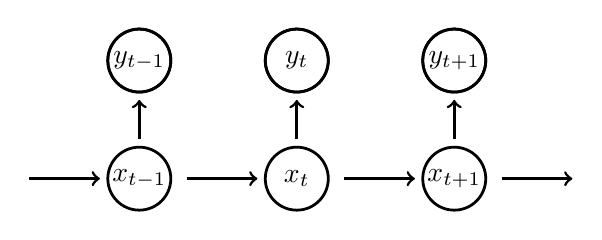
\begin{tikzpicture}[line width=1pt]
\foreach \x in {1,...,3} \draw (3+2*\x,0) circle (0.4cm);
\foreach \x in {1,...,3} \draw (3+2*\x,1.5) circle (0.4cm);
\foreach \x in {1,...,3} \draw (3+2*\x,1.5) circle (0.4cm);
\foreach \x in {1,...,3} \draw [<-] (3+2*\x, 1) -- (3+2*\x,.5);
\foreach \x in {1,...,4} \draw [->] (3+2*\x-1.4, 0) -- (3+2*\x-.5,0);
\draw (3+2*1,0) node {$x_{t-1}$};
\draw (3+2*2,0) node {$x_{t}$};
\draw (3+2*3,0) node {$x_{t+1}$};
\draw (3+2*1,1.5) node {$y_{t-1}$};
\draw (3+2*2,1.5) node {$y_{t}$};
\draw (3+2*3,1.5) node {$y_{t+1}$};
\end{tikzpicture}
\end{figure}
}

\frame{\frametitle{Sequential estimation in state-space models} \pause
Joint likelihood \pause
\begin{itemize}
\item $p(y_{1:t},x_{0:t},\theta) = p(y_t|x_t,\theta)p(x_t|x_{t-1},\theta)p(y_{1:t-1},x_{0:t-1},\theta)$
\end{itemize} \pause
Filtered distributions \pause
\begin{itemize}
\item $p(x_{0:t},\theta|y_{1:t}) \propto p(y_t|x_t,\theta)p(x_t|x_{t-1},\theta)p(x_{0:t-1},\theta|y_{1:t-1})$ \pause
\item $p(x_t,\theta| y_{1:t}) \propto \int p(y_t|x_t,\theta)p(x_t|x_{t-1},\theta)p(x_{t-1},\theta|y_{1:t-1})\mbox{d}x_{t-1}$ \pause
\end{itemize}
Smoothed distributions: $p(x_s,\theta|y_{1:t})$ for any $s < t$ \pause
\begin{itemize}
\item $p(x_s,\theta|y_{1:t}) = \int_{x_{0:s-1}} \int_{x_{s+1:t}} p(x_{0:t},\theta|y_{1:t},)\mbox{d}x_{0:s-1}\mbox{d}x_{s+1:t}$ \pause
\end{itemize}
Marginal likelihood of the data: $p(y_{1:t})$ \pause
\begin{itemize}
\item $p(y_{1:t}) = \int_{\theta} \int_{x_{0:t}} p(y_{1:t},x_{0:t},\theta)\mbox{d}x_{0:t}\mbox{d}\theta$ \pause
\end{itemize}
Analytical tractability only in special cases
}

\frame{\frametitle{State-space model of an epidemic} \pause
Modeling disease transmission: \pause
\begin{itemize}
\item SIR model \pause
\item keep track of \% of population susceptible ($s_t$), infected ($i_t$), and recovered ($r_t$) at each day $t = 0,1,2,\ldots,T$ \pause
\item fixed population size $P$ \pause
\item $s_t + i_t + r_t = 1$ \pause
\item $x_t = (s_t,i_t)$ - unobserved state of the epidemic at day $t$ \pause
\item fixed parameters $\beta > 0$, $\gamma > 0$, and $\nu > 0$: \pause
\item $\beta =$ rate of spread \pause
\item $\gamma =$ recovery time from infection \pause
\item $\nu =$ population mixing intensity \pause
\item $\theta = (\beta, \gamma, \nu)'$
\end{itemize}
}

\frame{\frametitle{State-space model of an epidemic}
State equation: \pause
\[x_{t+1}\left|x_t,\theta\right. \sim \mbox{N}_\Omega\left(f(x_t,\theta),Q(\theta)\right),\]
where
\[f(x_t,\theta) = \left(
\begin{array}{c}
s_t - \beta i_ts^\nu_t \phantom{- \gamma i_t}\,\, \\
i_t +  \beta i_ts^\nu_t - \gamma i_t
\end{array}
\right),
\qquad
Q(\theta) = \frac{\beta}{P^2} \left(
\begin{array}{ccccc}
1 & -1 \\
-1 & 1 + \gamma/\beta
\end{array}
\right),\]
$\Omega = \{(s_t,i_t): s_t \ge 0, i_t \ge 0, s_t + i_t \le 1\}$, and \\ \pause
$p(x_0,\theta) = p(i_0)\delta_{1-i_0}(s_0)p(\theta)$ with $i_0 \sim \mbox{N}_{[0,1]}(0.002,0.0005^2)$ \pause
\begin{itemize}
\item \citet{skvortsov2012monitoring,sheinson:niemi:meiring:epidtrack:2014} \pause
\item \citet{herwaarden1995stochepid,dangerfield2009stochepid,anderson2004sars}
\end{itemize}
}

\frame{\frametitle{State-space model of an epidemic}
\begin{itemize}
\item $R_0 = \frac{\beta}{\gamma}$ - basic reproductive number \pause
\item seasonal flu - $R_0 \approx 1.5$, polio - $R_0 \approx 5$, chicken pox - $R_0 \approx 10$
\end{itemize} \pause
\includegraphics[width=0.45\textwidth]{sircurves1} \pause
\includegraphics[width=0.45\textwidth]{sircurves2}
}

\frame{\frametitle{State-space model of an epidemic}
Observation equation: \pause
\begin{itemize}
\item observe syndromic data from $L$ streams \pause
\item $y_{l,t}$ - observed data from stream $l$ at day $t$ \pause
\item e.g. counts of flu-related internet search queries, emergency room visits, etc. \pause
\item $y_t = (y_{1,t},y_{2,t},\ldots,y_{L,t})'$ be observed data at day $t$, $t=1,2,\ldots,T$ \pause
\item assume a stochastic power-law relationship between $\log y_t$ and $i_t$, i.e.
\[\log y_{l,t} |x_t,\theta \sim \mbox{N}\left(b_li_t^{\varsigma_l}+\eta_l,\sigma_l^2\right)\] \pause
\item \citet{Gins:Mohe:Pate:Bram:Smol:Bril:dete:2009}, \citet{skvortsov2012monitoring} \pause
\item initially assume $L = 4$ and $\eta_l$, $b_l$, $\varsigma_l$, and $\sigma_l$ known for all $l$ \pause
\item extended analysis: $L = 1$ and $\theta = (\beta,\gamma,\nu,b,\varsigma,\sigma,\eta)'$
\end{itemize}
}

\frame{\frametitle{Dynamic linear models (DLMs)} \pause
\begin{align*}
y_t &= U_t\beta + F_tx_t + v_t, &\quad v_t \stackrel{iid}{\sim} \mbox{N}(0,V) \\
x_t &= Gx_{t-1} + w_t, &\quad w_t \stackrel{iid}{\sim} \mbox{N}(0,W) \\
x_0 &\sim \mbox{N}(m_0, C_0) &
\end{align*} \pause
\begin{itemize}
\item $y_t: q \times 1 \quad v_t: q \times 1 \quad V: q \times q$ \pause
\item $x_t: p \times 1 \quad w_t: p \times 1 \quad W: p \times p$  \pause
\item $F_t: q \times p \quad G: p \times p$ \pause
\item $U_t: q \times d \quad \beta: d \times 1$ \pause
\item $m_0: p \times 1 \quad C_0: p \times p$ \pause
\item $v_s \perp w_s'$ for all $s \ne s'$ \pause
\item assume univariate $y_t$, i.e. $q = 1$ \pause
\item $G$, $V$, $W$, $C_0$, and $\beta$ could contain unknown fixed parameters
\end{itemize}
}

\frame{\frametitle{Dynamic linear models (DLMs)}
Analytical tractability if all fixed parameters known \pause \\
Filtered distributions $x_t|y_{1:t} \sim \mbox{N}(m_t,C_t)$ for $t=1,\ldots,T$, where
\begin{align*}
z_t &= Gm_{t-1} &\qquad R_t &= GC_{t-1}G' + W \\
f_t &= F_tz_t + U_t\beta &\qquad Q_t &= F_tR_tF_t' + V \\
m_t &= z_t + R_tF_t'Q_t^{-1}(y_t-f_t) &\qquad C_t &= R_t - R_tF_t'Q_t^{-1}F_tR_t
\end{align*} \pause
Smoothed distributions $x_t|y_{1:T} \sim \mbox{N}(h_t,H_t)$ for any $t < T$, where
\begin{align*}
h_t &= m_t + C_tG'R_{t+1}^{-1}(h_{t+1} - z_{t+1}) \\
H_t &= C_t - C_tG'R_{t+1}^{-1}(R_{t+1} - H_{t+1})R_{t+1}^{-1}GC_t
\end{align*}
with $h_T = m_T$ and $H_T = C_T$ \pause \\
Recursions known as Kalman filter and Kalman smoother \citep{kal:1960:ekf,petris:camp:2009:dynamic}
}

\frame{\frametitle{First-order DLM with common variance factor} \pause
Let $F_t = G = 1$, $p = 1$, $V = \theta$, and $\theta\lambda$ \pause
\begin{align*}
y_t &\sim \mbox{N}(x_t, \theta) \\
x_t &\sim \mbox{N}(x_{t-1}, \theta\lambda)
\end{align*} \pause
\begin{itemize}
\item prior: $x_0|\theta \sim \mbox{N}(0, \theta) \quad \theta \sim \mbox{IG}(a_0,b_0)$ \pause
\item $\theta$ - unknown common state and observation variance factor \pause
\item $\lambda$ - signal-to-noise ratio, assumed known \pause
\item $a_0$ and $b_0$ assumed known
\end{itemize}
}

\frame{\frametitle{First-order DLM with common variance factor}
Analytically tractable filtered distributions \pause \\
$x_t|\theta,y_{1:t} \sim \mbox{N}(m_t,\theta c_t) \quad \theta|y_{1:t} \sim \mbox{IG}(a_t, b_t) \quad x_t|y_{1:t} \sim \mbox{T}\left(m_t,c_t \frac{b_t}{a_t},2a_t\right)$, \pause
where $m_t$, $c_t$, $a_t$, and $b_t$ are calculated recursively according to
\begin{align*}
f_t &= m_{t-1} &\qquad q_t &= c_{t-1} + \lambda + 1 \\
m_t &= (1 - c_t)f_t + c_ty_t &\qquad c_t &= 1 - \frac{1}{q_t} \\
a_t &= a_{t-1} + \frac{1}{2} &\qquad b_t &= b_{t-1} + \frac{(y_t-f_t)^2}{2q_t}
\end{align*}
starting with $m_0 = 0$, $c_0 = 1$, and known $a_0$ and $b_0$ \pause \\
Analytically tractable marginal likelihood $p(y_{1:t})$ \pause \\
$y_t|y_{1:t-1} \sim \mbox{T}\left(f_t,q_t\frac{b_{t-1}}{a_{t-1}},2a_{t-1}\right) \quad p(y_{1:t}) = \left(\prod_{k=2}^t p(y_k|y_{1:k-1})\right)p(y_1)$ \\
$y_1 \sim \mbox{T}(f_1,q_1b_0/a_0,2a_0)$
}

\frame{\frametitle{Regression with ARMA errors} \pause
$y_t = U_t\beta + x_t$, where, $x_t$ follows a zero-mean $\mbox{ARMA}(P, Q)$ stochastic process \pause \\
\[
\begin{array}{ccc}
x_t &= & (x_{t,1} ,x_{t,2}, \ldots, x_{t,m})' \\
m &= & \mbox{max}(P,Q+1) \\ \pause
F_t &= & (1,0,\ldots,0)_{1\times m} \\ \pause
v_t &= & 0 \\ \pause
W &= & \sigma^2ee' \\
e &= & (1, \gamma_1, \ldots, \gamma_{m-1})' \pause
\end{array} \quad
G = \left(
 \begin{array}{ccccc}
 \phi_1 & \vdots \\
 \phi_2 & \vdots \\
 \phi_3 & \vdots && I_{m-1} \\
 \vdots & \vdots \\
 \cdots & \cdots & \cdots & \cdots & \cdots \\
 \phi_m &\vdots & 0 & \cdots & 0
 \end{array}
\right)\] \pause
$\phi_s = 0$ for $s > P$ and $\gamma_r = 0$ for $r > Q$ \pause \\
$y_t = U_t\beta + \phi_1x_{t-1,1} + \cdots + \phi_Px_{t-P,1} + \epsilon_t + \gamma_1\epsilon_{t-1} + \cdots + \gamma_Q\epsilon_{t-Q}$,
where $t \ge m$ and $\epsilon_j \stackrel{iid}{\sim} \mbox{N}(0,\sigma^2)$ for $j \ge 0$
}

\frame{\frametitle{Regression with ARMA errors}
Stationarity: \pause roots of $\phi(z)$ lie outside of unit circle, where
\[\phi(z) = 1 - \phi_1z - \phi_2z^2 - \cdots - \phi_Pz^P \label{eqn:arpoly}\] \pause
Invertibility: roots of $\gamma(z)$ lie outside of unit circle, where
\[\gamma(z) = 1 + \gamma_1z + \gamma_2z^2 + \cdots + \gamma_Qz^Q\] \pause
Stationary presample errors: \pause
\[x_0 \sim \mbox{N}(0, \sigma^2\Omega),\]
where $\mbox{vec}(\Omega) = (I_{m^2} - G\otimes G)^{-1} \mbox{vec}(ee')$ \\ \pause
Example: regression with AR(1) errors \\ \pause
Set: $m = P = 1$, $Q = 0$, $F_t = 1$, $W = \sigma^2$, $G = \phi$ \\ \pause
Model: $y_t = U_t\beta + x_t  \quad x_t = \phi x_{t-1} + \epsilon_t \quad \ t \ge 1$ \\ \pause
Stationarity: $-1 < \phi < 1$, $x_0 \sim \mbox{N}(0, \sigma^2 / (1 - \phi^2))$
}

\frame{\frametitle{Dynamic regression models} \pause
\begin{align*}
y_t &= U_t\beta + F_tx_t + v_t, &\quad v_t \stackrel{iid}{\sim} \mbox{N}(0,V) \\
x_t &= Gx_{t-1} + w_t, &\quad w_t \stackrel{iid}{\sim} \mbox{N}(0,W)
\end{align*} \pause
Let $x_t$ follow an AR(1) process, i.e. $W = \sigma^2_s$ and $G = \phi$ \pause \\
Let $V = \sigma^2_m$, $U_t = (1,u_t)$, and $\beta = (\beta_0,\beta_1)'$ \pause \\
Let $p(x_0) = \delta_{0}(x_0)$ \pause \\
Dynamic intercept model: $F_t = 1$ for all $t$ \pause \\
\[y_t = (\beta_0 + x_t) + \beta_1u_t + v_t, \ v_t \stackrel{iid}{\sim}\mbox{N}(0,\sigma^2_m)\] \pause
Dynamic slope model: $F_t = u_t$ \pause \\
\[y_t = \beta_0 + (\beta_1 + x_t)u_t + v_t, \ v_t \stackrel{iid}{\sim}\mbox{N}(0,\sigma^2_m)\] \pause
Unknown fixed parameters $\theta = (\beta',\phi,\sigma^2_s,\sigma^2_m)'$
}

\frame{\frametitle{Dynamic regression models}
Dynamic intercept and slope model $M_{111}$: \pause
\[F_t = (1, u_t) \quad G = \left(\begin{array}{cc} \phi & 0 \\ 0 & \rho \end{array}\right) \quad W = \left(\begin{array}{cc} \sigma^2_s & 0 \\ 0 & \sigma^2_b \end{array}\right)\] \pause
\begin{align*}
y_t &= (\beta_0 + x_{t,1}) + (\beta_1 + x_{t,2})u_t + v_t, \ v_t \stackrel{iid}{\sim} \mbox{N}(0,\sigma^2_m) \\
x_{t,1} &= \phi x_{t-1,1} + w_{t,1}, \ w_{t,1} \stackrel{iid}{\sim} \mbox{N}(0,\sigma^2_s) \\
x_{t,2} &= \rho x_{t-1,2} + w_{t,2}, \ w_{t,2} \stackrel{iid}{\sim} \mbox{N}(0,\sigma^2_b)
\end{align*} \pause
Unknown fixed parameters $\theta = (\beta',\phi,\rho,\sigma^2_s,\sigma^2_b,\sigma^2_m)'$
}

\frame{\frametitle{Dynamic regression models}
Model notation: $M_{ijk}$ \pause
\begin{itemize}
\item $i$ is AR order of change in intercept
\item $j$ is AR order of change in slope
\item $k$ is 1 or 0 indicating whether additional measurement noise is included
\end{itemize} \pause
Dynamic intercept model: $M_{101}$ \\ \pause
Dynamic slope model: $M_{011}$ \\ \pause
Dynamic intercept and slope model: $M_{111}$ \\ \pause
Regression with AR(1) errors: $M_{100}$ \\ \pause
Simple linear regression: $M_{001}$
}

\section{Monte Carlo estimation \label{sec:def:est}}

\frame{\frametitle{Monte Carlo approximation}
What if $p(x_t,\theta|y_{1:t})$ cannot be calculated? \\ \pause
Sample-based approximations \\ \pause
Markov chain Monte Carlo (MCMC) \pause
\begin{itemize}
\item provides smoothed estimates of states in state-space models \pause
\item inefficient for sequential analysis \pause
\end{itemize}
Sequential Monte Carlo (SMC), a.k.a. particle filtering \pause
\begin{itemize}
\item updates estimates on-line \pause
\item direct estimates of marginal likelihood \pause
\item inefficient for smoothing
\end{itemize}
}

\frame{\frametitle{Particle filtering} \pause
Based on a sequential use of important sampling \\ \pause
Approximates $p(x_t,\theta|y_{1:t})$ through a weighted Monte Carlo realization in terms of $J$ particles, i.e.
\[p(x_t,\theta| y_{1:t}) \approx \sum_{j=1}^J w_t^{(j)} \delta_{\left(x_t^{(j)},\theta^{(j)}\right)}(x_t,\theta)\] \pause
\begin{itemize}
\item $\left(x_t^{(j)},\theta^{(j)}\right)$ - location of the $j^{\mbox{th}}$ particle at time $t$ \pause
\item $w_t^{(j)}$ - weight of particle $j$ with $\sum_{j=1}^J w_t^{(j)}=1$ \pause
\end{itemize}
}

\frame{\frametitle{Bootstrap filter (BF) \citep{Gord:Salm:Smit:nove:1993,Kita:mont:1996}} \pause
Assume $\theta$ known \\ \pause
Given an approximation to $p(x_t|y_{1:t})$, move to an approximation to $p(x_{t+1}|y_{1:t+1})$ by the following steps for each particle $j=1,\ldots,J$:
\begin{enumerate}
\item Resample: sample an index $k\in\{1,\ldots,j,\ldots,J\}$ with associated probabilities $\left\{w_t^{(1)},\ldots,w_t^{(j)},\ldots,w_t^{(J)}\right\}$, \pause
\item Propagate: sample $x_{t+1}^{(j)} \sim p\left( x_{t+1}\left|x_t^{(k)}\right.\right)$, and \pause
\item Calculate weights and renormalize:
\[ \tilde{w}_{t+1}^{(j)} = p\left(y_{t+1}\left|x_{t+1}^{(j)}\right.\right) \qquad w_{t+1}^{(j)} = \tilde{w}_{t+1}^{(j)}\left/ \sum_{l=1}^J \tilde{w}_{t+1}^{(l)} \right. .\] \pause
\end{enumerate}
Apply recursively \\ \pause
Initial weights $w_0^{(j)}$ and locations $x_0^{(j)}$ for all $j$ \\ \pause
Sample from $p(x_0)$ with uniform weights
}

\frame{\frametitle{Auxiliary particle filter (APF) \citep{Pitt:Shep:filt:1999}} \pause
Problem: $w_t^{(j)}$ small for particles for which $p\left(y_{t}\left|x_{t}^{(j)}\right.\right)$ is small \\ \pause
Solution: look ahead for particles with higher likelihood using $y_{t+1}$ \\ \pause
\begin{enumerate}
\item For each particle $j$, calculate a point estimate of $x_{t+1}^{(j)}$ called $\mu_{t+1}^{(j)}$ \pause
\item Calculate auxiliary weights: $\tilde{g}_{t+1}^{(j)} = w_t^{(j)} p\left(y_{t+1}\left|\mu_{t+1}^{(j)}\right.\right)$ \pause
\item Renormalize weights: $g_{t+1}^{(j)} = \tilde{g}_{t+1}^{(j)}\left/\sum_{l=1}^J \tilde{g}_{t+1}^{(l)}.\right.$ \pause
\item For each particle $j=1,\ldots,J$,
	\begin{enumerate}
    \item Resample: sample an index $k\in\{1,\ldots,j,\ldots,J\}$ with associated probabilities \pause $\left\{g_{t+1}^{(1)},\ldots,g_{t+1}^{(j)},\ldots,g_{t+1}^{(J)}\right\}$,
	\item Propagate: sample $x_{t+1}^{(j)} \sim p\left(x_{t+1}\left|x_t^{(k)}\right.\right)$, and \pause
	\item Calculate weights: $\tilde{w}_{t+1}^{(j)} = p\left(y_{t+1}\left|x_{t+1}^{(j)}\right.\right) \left/ p\left(y_{t+1}\left|\mu_{t+1}^{(k)}\right.\right)\right.$ \pause
    \item Renormalize: $w_{t+1}^{(j)} = \tilde{w}_{t+1}^{(j)}\left/\sum_{l=1}^J \tilde{w}_{t+1}^{(l)}. \right.$ \pause
	\end{enumerate}
\end{enumerate}
Typically $\mu_{t+1}^{(j)} = E\left(x_{t+1}\left|x_t^{(j)} \right.\right)$
}

\frame{\frametitle{Kernel density particle filter (KDPF) \citep{Liu:West:comb:2001}} \pause
Problem: $\theta$ must be included in $x_t$ \pause $\Rightarrow$ degeneracy in unique fixed parameter values \\ \pause
Solution: regenerate $\{\theta_t^{(1)},\ldots,\theta_t^{(J)}\}$ from a kernel density approximation to $p(\theta|y_{1:t})$ \\ \pause
Mixture of normals:
\[p(\theta|y_{1:t}) \approx \sum_{j=1}^J w_t^{(j)}\mbox{N}(m_t^{(j)}, h^2V_t),\] \pause
\begin{align*}
m_t^{(j)} &= a\theta_t^{(j)} + (1-a)\bar{\theta}_t \\
\bar{\theta}_t &= \mbox{ sample mean of } \theta_t^{(1)},\ldots,\theta_t^{(J)} \\
V_t &= \mbox{ sample covariance of } \theta_t^{(1)},\ldots,\theta_t^{(J)} \\ \pause
a^2 &= 1 - h^2 \\
h^2 &= 1 - ((3\Delta - 1)/2\Delta)^2 \\
\Delta &= \mbox{ discount factor } \in [0.95,0.99]
\end{align*} \pause
Reparameterize $\theta$ to the real line
}

\frame{\frametitle{Kernel density particle filter (KDPF) \citep{Liu:West:comb:2001}}
\begin{enumerate}
\item For each particle $j$, set $m_t^{(j)} = a\theta_t^{(j)} + (1-a)\bar{\theta}_t$ and calculate a point estimate of $x_{t+1}^{(j)}$ called $\mu_{t+1}^{(j)}$ \pause
\item Calculate auxiliary weights: $\tilde{g}_{t+1}^{(j)} = w_t^{(j)} p\left(y_{t+1}\left|\mu_{t+1}^{(j)},m_t^{(j)}\right.\right)$ \pause
\item Renormalize: $g_{t+1}^{(j)} = \tilde{g}_{t+1}^{(j)}\left/ \sum_{l=1}^J \tilde{g}_{t+1}^{(l)}. \right.$ \pause
\item For each particle $j=1,\ldots,J$,
	\begin{enumerate}
    \item Resample: sample an index $k\in\{1,\ldots,j,\ldots,J\}$ with associated probabilities $\left\{g_{t+1}^{(1)},\ldots,g_{t+1}^{(j)},\ldots,g_{t+1}^{(J)}\right\}$, \pause
	\item Regenerate the fixed parameters: sample $\theta_{t+1}^{(j)} \sim \mbox{N}\left(m_t^{(k)}, h^2V_t \right)$, \pause
	\item Propagate: sample $x_{t+1}^{(j)} \sim p\left(x_{t+1}\left|x_t^{(k)},\theta_{t+1}^{(j)}\right.\right)$, and \pause
	\item Calculate weights: $\tilde{w}_{t+1}^{(j)} = p\left(y_{t+1}\left|x_{t+1}^{(j)},\theta_{t+1}^{(j)}\right.\right)\left/p\left(y_{t+1}\left|\mu_{t+1}^{(k)},m_t^{(k)}\right.\right)\right.$ \pause
    \item Renormalize: $w_{t+1}^{(j)} = \tilde{w}_{t+1}^{(j)}\left/\sum_{l=1}^J \tilde{w}_{t+1}^{(l)}. \right.$ \pause
	\end{enumerate}
\end{enumerate}
}

\frame{\frametitle{Resample-move particle filter (RM) \citep{Gilk:Berz:foll:2001}} \pause
Regenerate fixed parameter values using a kernel closer to $p(\theta|y_{1:t})$ \\ \pause
\begin{itemize}
\item MCMC transition kernel $q$ with stationary distribution equal to $p(\theta|y_{1:t})$ \\ \pause
\item Define $x_{0:t}^{(j)} = \left(x_0^{(j)},x_1^{(j)},\ldots,x_t^{(j)}\right)$ and represent particle $j$ by $\left(x_{0:t}^{(j)},\theta_t^{(j)}\right)$ \\ \pause
\item $q$ satisfies $\int_{\theta}\int_{x_{0:t}} p(x_{0:t},\theta|y_{1:t})q\left(x_{0:t}^*,\theta^*|x_{0:t}^{(j)},\theta_t^{(j)}\right)\mbox{d}x_{0:t}\mbox{d}\theta = p(x_{0:t},\theta|y_{1:t})$ \\ \pause
\item $\left(x_{0:t}^{(j)},\theta_t^{(j)}\right) \stackrel{.}{\sim} p(x_{0:t},\theta|y_{1:t})$ implies $\left(x_{0:t}^*,\theta^*\right)$ drawn from $q\left(x_{0:t},\theta|x_{0:t}^{(j)},\theta_t^{(j)}\right)$ can only have distribution closer to  $p(x_{0:t},\theta|y_{1:t})$ \pause
\item $\theta^*$ has distribution closer to $p(\theta|y_{1:t})$
\end{itemize}
}

\frame{\frametitle{Resample-move particle filter (RM) \citep{Gilk:Berz:foll:2001}}
Given a particle approximation to $p(x_{0:t},\theta|y_{1:t})$, move to a particle approximation to $p(x_{0:t+1},\theta|y_{1:t+1})$ by the following for each particle $j=1,\ldots,J$: \pause
\begin{enumerate}
\item Propagate: draw $\tilde{x}^{(j)}_{t+1}$ from $p\left(x_{t+1}|x^{(j)}_t,\theta^{(j)}_t\right)$. Incorporate $\tilde{x}^{(j)}_{t+1}$ into particle $j$ and denote the new augmented particle by $\left(\tilde{x}^{(j)}_{0:t+1},\theta^{(j)}_t\right)$, \pause
\item Calculate weights: $\tilde{w}^{(j)}_t = p\left(y_{t+1}|\tilde{x}^{(j)}_{t+1},\theta^{(j)}_t\right)$ \pause 
\item Renormalize: $w^{(j)}_{t+1} = \tilde{w}_{t+1}^{(j)}\left/\sum_{l=1}^J \tilde{w}_{t+1}^{(l)}, \right.$ \pause
\item Resample: sample an index $k$ from $\{1,\ldots,j,\ldots,J\}$ with associated probabilities $\{w^{(1)}_{t+1},\ldots,w^{(j)}_{t+1},\ldots,w^{(J)}_{t+1}\}$, and \pause
\item \label{step:move} Move particles: draw a new particle $\left(x^{(j)}_{0:t+1},\theta^{(j)}_{t+1}\right) \sim q\left(x_{0:t+1},\theta|\tilde{x}^{(k)}_{0:t+1},\theta^{(k)}_t\right)$ with invariant distribution $p(x_{0:t+1},\theta|y_{1:t+1})$.
\end{enumerate}
}

\frame{\frametitle{RM example - first-order DLM} \pause
\begin{align*}
y_t &\sim \mbox{N}(x_t, \theta) \\
x_t &\sim \mbox{N}(x_{t-1}, \theta\lambda) \\
x_0|\theta &\sim \mbox{N}(0, \theta) \quad \theta \sim \mbox{IG}(a_0,b_0)
\end{align*} \pause
Sample from $q$ as follows: For a given particle $j$ and sampled index $k$,
\begin{enumerate}
\item \label{step:move:ll} Sample $\theta^{(j)}_{t+1}$ conditional on $\tilde{x}_{0:t+1}^{(k)}$ from $\mbox{IG}(a_t, b_t)$, where
\begin{align*}
a_t &= a_0 + 1/2 + t \\
b_t &= b_0 + \frac{1}{2}\left(\sum_{i=1}^t \left(y_i - \tilde{x}_i^{(k)}\right)^2 + \frac{1}{\lambda}\sum_{i=1}^t \left(\tilde{x}_i^{(k)} - \tilde{x}_{i-1}^{(k)}\right)^2 + \left(\tilde{x}^{(k)}_0\right)^2\right)
\end{align*} \pause
\item Sample $x_{0:t+1}^{(j)}$ conditional on $\theta^{(j)}_{t+1}$ via forward filtering backward sampling (FFBS), based on Kalman filter and smoother recursions with
\[m_0 = 0 \quad C_0 = V = \theta^{(j)}_{t+1} \quad W = \theta_{t+1}^{(j)}\lambda \quad F_t = G = 1.\]
\end{enumerate}
}

\frame{\frametitle{Particle learning (PL) \citep{Carv:Joha:Lope:Pols:part}} \pause
Increases efficiency by regenerating $\theta$ using sufficient statistics $s_t$ \\ \pause
\begin{align*}
p(x_{t+1},s_{t+1},\theta|y_{1:t+1}) \propto & \int_{s_t}\int_{x_t} p(s_{t+1}|y_{t+1},x_{t+1},s_t)p(x_{t+1}|y_{t+1},x_t,\theta) \\
& p(y_{t+1}|x_t,\theta)p(x_t,s_t,\theta|y_{1:t})\mbox{d}x_t\mbox{d}s_t \pause
\end{align*}
\begin{itemize}
\item incorporates look ahead strategy through $p(y_{t+1}|x_t,\theta)$ \pause
\item propagates states through $p(x_{t+1}|y_{t+1},x_t,\theta)$ \pause
\item sequential algorithm through tracking sufficient statistics for $\theta$ \pause
\item must be able to sample from $p(\theta|s_t)$ and $p(x_{t+1}|y_{t+1},x_t,\theta)$ \pause
\item must be able to evaluate $p(y_{t+1}|x_t,\theta)$ up to a constant \pause
\item must be able to update $s_{t+1}$ given $s_t$, $x_{t+1}$, and $y_{t+1}$ \pause
\item incorporate sufficient statistics into particles, i.e. location of particle $j$ at time $t$ is $\left(x^{(j)}_t,\theta^{(j)}_t,s_t^{(j)}\right)$
\end{itemize}
}

\frame{\frametitle{Particle learning (PL) \citep{Carv:Joha:Lope:Pols:part}}
We move from an approximation to $p(x_t,\theta|y_{1:t})$ to that of $p(x_{t+1},\theta|y_{1:t+1})$ by the following procedure for each particle $j = 1,2,\ldots,J$:
\begin{enumerate}
\item Calculate weights: $\tilde{w}_{t+1}^{(j)} = p\left(y_{t+1}\left|x_t^{(j)},\theta_t^{(j)}\right.\right)$ \pause
\item Renormalize: $w_{t+1}^{(j)} = \tilde{w}_{t+1}^{(j)} \left/ \sum_{l=1}^J \tilde{w}_{t+1}^{(l)}\right.$ \pause
\item Resample: sample an index $k \in \{1,\ldots,j,\ldots,J\}$ with associated probabilities $\{w_{t+1}^{(1)},\ldots,w_{t+1}^{(j)},\ldots,w_{t+1}^{(J)}\}$, \pause
\item Propagate: sample $x_{t+1}^{(j)} \sim p\left(x_{t+1}\left|y_{t+1},x_t^{(k)},\theta_t^{(k)}\right.\right)$, \pause
\item Update sufficient statistics: calculate $s_{t+1}^{(j)} = S\left(y_{t+1},x_{t+1}^{(j)},s_t^{(k)}\right)$, and \pause
\item Regenerate: sample $\theta_{t+1}^{(j)} \sim p\left(\theta\left|s_{t+1}^{(j)}\right.\right)$.
\end{enumerate}
}

\section{Results \label{sec:def:results}}

\frame{\frametitle{References}
\bibliographystyle{plainnat}
{\tiny
\bibliography{danny}
}
}

\end{document}